\documentclass[border=10pt]{standalone}

\usepackage{tikz}
\usetikzlibrary{decorations.markings,calc,arrows}

% Load style for signal-flow graphs
%%%
%%% For the SFGs
%%%
\tikzset{%
	% Style of the node
	Node/.style={circle,thick,draw=black,inner sep=0, minimum size=0.15cm},
	% Style of the node label
	NodeName/.style={font=\footnotesize,black,outer sep=1},
	% Style of the branche label
	ArrowName/.style={font=\footnotesize,auto,outer sep=1},
	% Style of the branch
	Connection/.style={thick},
	->-/.style={decoration={
			markings,
			mark=at position #1 with {\draw[->,>=latex',line width=2pt](0pt,0)--(4pt,0);}},
		postaction={decorate}},
	->-/.default=0.50,
	MarkMiddle/.style={decoration={
			markings,
			mark=at position 0.5 with {\node[NodeName](middle_#1){};}},
		postaction={decorate}},
}

\begin{document}
	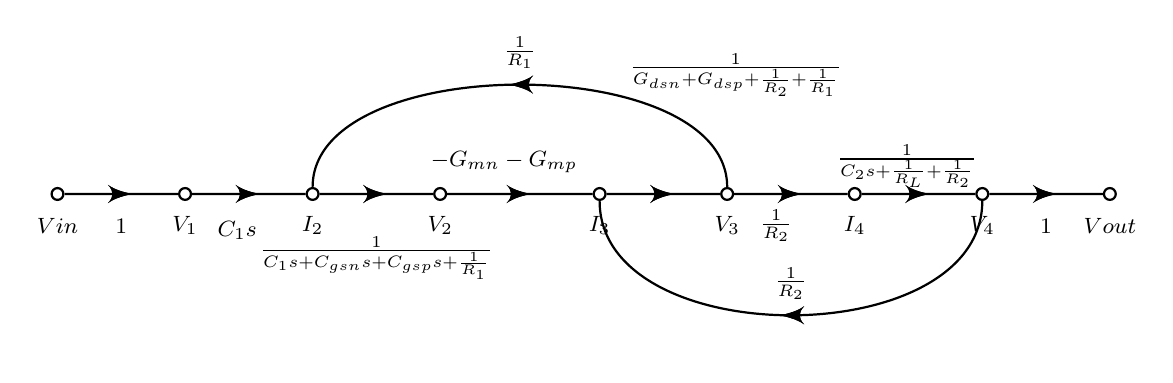
\begin{tikzpicture}[scale = 0.3,x=0.045cm,y=-0.045cm] % STYLES


%~~~~~~~~~~~~~~~~~~~~~~~~~~~~~~~~~~~~~~~~~~~~~~~~~~
% Set Nodes
%~~~~~~~~~~~~~~~~~~~~~~~~~~~~~~~~~~~~~~~~~~~~~~~~~~
\node[Node] (N1) at (531, 239) {};
\node[NodeName] at ($ (N1) + (0, 30) $) {$I_{3}$};

\node[Node] (N2) at (141, 239) {};
\node[NodeName] at ($ (N2) + (0, 30) $) {$V_{1}$};

\node[Node] (N3) at (21, 239) {};
\node[NodeName] at ($ (N3) + (0, 30) $) {$Vin$};

\node[Node] (N4) at (771, 239) {};
\node[NodeName] at ($ (N4) + (0, 30) $) {$I_{4}$};

\node[Node] (N5) at (381, 239) {};
\node[NodeName] at ($ (N5) + (0, 30) $) {$V_{2}$};

\node[Node] (N6) at (651, 239) {};
\node[NodeName] at ($ (N6) + (0, 30) $) {$V_{3}$};

\node[Node] (N7) at (261, 239) {};
\node[NodeName] at ($ (N7) + (0, 30) $) {$I_{2}$};

\node[Node] (N8) at (891, 239) {};
\node[NodeName] at ($ (N8) + (0, 30) $) {$V_{4}$};

\node[Node] (N9) at (1011, 239) {};
\node[NodeName] at ($ (N9) + (0, 30) $) {$Vout$};



%~~~~~~~~~~~~~~~~~~~~~~~~~~~~~~~~~~~~~~~~~~~~~~~~~~
% Set Branches
%~~~~~~~~~~~~~~~~~~~~~~~~~~~~~~~~~~~~~~~~~~~~~~~~~~
%Branch from Node N5 to Node N1
\draw [->-, Connection, MarkMiddle=1] (N5) ..controls(426.0, 239.0) and (486.0, 239.0) .. (N1);
\node[ArrowName] at($ (middle_1) + (-15.0, -30.0) $) {$- G_{mn} - G_{mp}$};

%Branch from Node N1 to Node N6
\draw [->-, Connection, MarkMiddle=2] (N1) ..controls(576.0, 239.0) and (606.0, 239.0) .. (N6);
\node[ArrowName] at($ (middle_2) + (68.0, -112.0) $) {$\frac{1}{G_{dsn} + G_{dsp} + \frac{1}{R_{2}} + \frac{1}{R_{1}}}$};

%Branch from Node N2 to Node N7
\draw [->-, Connection, MarkMiddle=3] (N2) ..controls(186.0, 239.0) and (216.0, 239.0) .. (N7);
\node[ArrowName] at($ (middle_3) + (-11.0, 34.0) $) {$C_{1} s$};

%Branch from Node N8 to Node N1
\draw [->-, Connection, MarkMiddle=4] (N8) ..controls(891.0, 389.0) and (531.0, 389.0) .. (N1);
\node[ArrowName] at($ (middle_4) + (0.0, -30.0) $) {$\frac{1}{R_{2}}$};

%Branch from Node N6 to Node N7
\draw [->-, Connection, MarkMiddle=5] (N6) ..controls(651.0, 104.0) and (261.0, 104.0) .. (N7);
\node[ArrowName] at($ (middle_5) + (0.0, -30.0) $) {$\frac{1}{R_{1}}$};

%Branch from Node N3 to Node N2
\draw [->-, Connection, MarkMiddle=6] (N3) ..controls(66.0, 239.0) and (96.0, 239.0) .. (N2);
\node[ArrowName] at($ (middle_6) + (0.0, 30.0) $) {$1$};

%Branch from Node N7 to Node N5
\draw [->-, Connection, MarkMiddle=7] (N7) ..controls(306.0, 239.0) and (336.0, 239.0) .. (N5);
\node[ArrowName] at($ (middle_7) + (0.0, 60.0) $) {$\frac{1}{C_{1} s + C_{gsn} s + C_{gsp} s + \frac{1}{R_{1}}}$};

%Branch from Node N4 to Node N8
\draw [->-, Connection, MarkMiddle=8] (N4) ..controls(816.0, 239.0) and (846.0, 239.0) .. (N8);
\node[ArrowName] at($ (middle_8) + (-11.0, -26.0) $) {$\frac{1}{C_{2} s + \frac{1}{R_{L}} + \frac{1}{R_{2}}}$};

%Branch from Node N6 to Node N4
\draw [->-, Connection, MarkMiddle=9] (N6) ..controls(696.0, 239.0) and (726.0, 239.0) .. (N4);
\node[ArrowName] at($ (middle_9) + (-14.0, 30.0) $) {$\frac{1}{R_{2}}$};

%Branch from Node N8 to Node N9
\draw [->-, Connection, MarkMiddle=10] (N8) ..controls(936.0, 239.0) and (966.0, 239.0) .. (N9);
\node[ArrowName] at($ (middle_10) + (0.0, 30.0) $) {$1$};



	\end{tikzpicture}
\end{document}